\chapter{Технологический раздел}
В этом разделе будет обоснован выбор языка программирования и среды разработки, рассмотрена диаграмма основных классов и разобран интерфейс, предлагаемый пользователю.

\section{Требования к программе} 
Программа должна предоставлять следующие возможности:
\begin{itemize}
	\item визуальное отображение сцены;
	\item перемещение объектов;
	\item выбор сцены;
	\item профилирование времени отрисовки кадра;
	\item настройку виртуальной геометрии;
	\item настройку куллинга;
	\item настройку сцены и объектов сцены;
\end{itemize}

\section{Выбор языка программирования и среды разработки}
Существует множество языков, а также сред программирования, многие из которых обладают достаточно высокой эффективностью, удобством и простотой в использовании.

Для разработки данной программы были выбраны языки C++ и Nvidia Cuda. Данный выбор обусловлен следующими факторами:

\begin{itemize}
	\item Cuda позволяет написать функции, которые будут выполняться на графическом ускорителе. Это один из немногих языков общего назначения, имеющих эту возможность (к примеру, GLSL предназначен только для написания шейдеров);
	\item Cuda - надмножество языка C++;
	\item объектные файлы C++ и Cuda компонуются;
	\item С++ позволяет реализовать некоторые идиомы программирования, которые полезны в данном проекте для производительности, например: статический полиморфизм, использование структур(POD), низкоуровневое взаимодействие с памятью (cudaMalloc, cudaMemcpy);
	\item трехмерные объекты, также как и математические абстракции, естественным образом представляются в виде структур, что позволяет легко и эффективно организовывать их взаимодействие, при этом сохраняется читаемый и легко изменяемый код;
	\item стандартная библиотека Thurst, представляющая инструментарий STL в виде c++, оптимизированный для работы на графическом ускорителе, используя чрезвычайную параллельность, сортирующие сети, и упаковку потоков (stream compaction);
	\item у меня есть опыт использования обоих языков.
\end{itemize}

В качестве среды разработки была CLion. Некоторые факторы по которым была выбрана данная среда.
\begin{enumerate}
	\item включает весь основной функционал: параллельная сборка, отладчик, поддержка точек останова, сборки и т.д;
	\item разработчики имеют возможность расширить любой функционал, включая компиляцию, отладку;
	\item поддерживает оба языка программирования;
	\item данная среда бесплатна для студентов;
\end{enumerate}

В конечном итоге стек используемых инструментов принимает вид:
\begin{enumerate}
	\item C++ / Cuda;
	\item gcc + nvcc;
	\item cmake;
	\item OpenGL для вывода растра на экран;
\end{enumerate}

\section{Структура программы}

Так при написании программы используется язык C++, он имеет сразу несколько парадигм. Так как упор программы делается на lockless многопоточность,
особое внимание уделено функциональной парадигме. Из за плохой нативной поддержки, и производительности объектно ориентированного кода, он в меньшей 
мере был использован на графическом ускорителе. Если полиморфизм и реализован, то только статический.

Написано большое количество вспомогательных структур, но они не запускаются на видеокарте и не обладают параллельностью.
Их использование не релевантно тематике работы.

Условно классы в программе можно разделить на несколько групп по выполняемым функциям.

Рассмотрим работу вызова отрисовки:
\begin{Verbatim}
void DrawCaller::draw(DrawCallArgs args_unculled, Image &image)
{
	// interface
	interface->log_fps();
	interface->log_before_culling(args_unculled.models.size());

	DrawCallArgs args;

	if (interface->is_culling_enabled()) {
		args = culler->cull(args_unculled,
		 		*args_unculled.base.camera_ptr);
	} else {
		args = args_unculled;
	}
	interface->log_after_culling(args.models.size());

	if (interface->is_virtual_geometry_enabled()) {
		virtual_geometry_manager->
		populate_virtual_models(args, image,
		 args_unculled);
	}

	// dispatch
	image_resetter->async_reset(image);
	size_t streams_to_use = std::min(args.models.size(),
	 (size_t)n_streams);
	for (size_t i = 0; i < streams_to_use; i++)
	{
		zfillers[i]->resize(image);
		zfillers[i]->async_reset();
	}

	for (size_t i = 0; i < args.models.size(); i++)
		zfillers[i % zfillers.size()]->async_zbuf(args, i);

	// sync
	for (size_t i = 0; i < streams_to_use; i++)
		zfillers[i]->await();
	image_resetter->await();

	auto zbuffers = get_z_buffers();
	// parallel dispatch and sync
	parallel_reduce_merge(z_mergers, zbuffers, 
	(int)streams_to_use);
	auto final_zbuffer = get_final_z_buffer();

	// dispatch
	for (size_t i = 0; i < args.models.size(); i++)
		rasterizers[i % rasterizers.size()]->async_rasterize(
			args,
			i, image, final_zbuffer);

	// sync
	for (size_t i = 0; i < streams_to_use; i++)
		rasterizers[i]->await();

	interface->draw_widget();
}
\end{Verbatim}
  

\section{Интерфейс}

На рисунке \ref{img:program_interface_basic} представлен интерфейс программы.

\begin{figure}[H]
	\begin{center}
		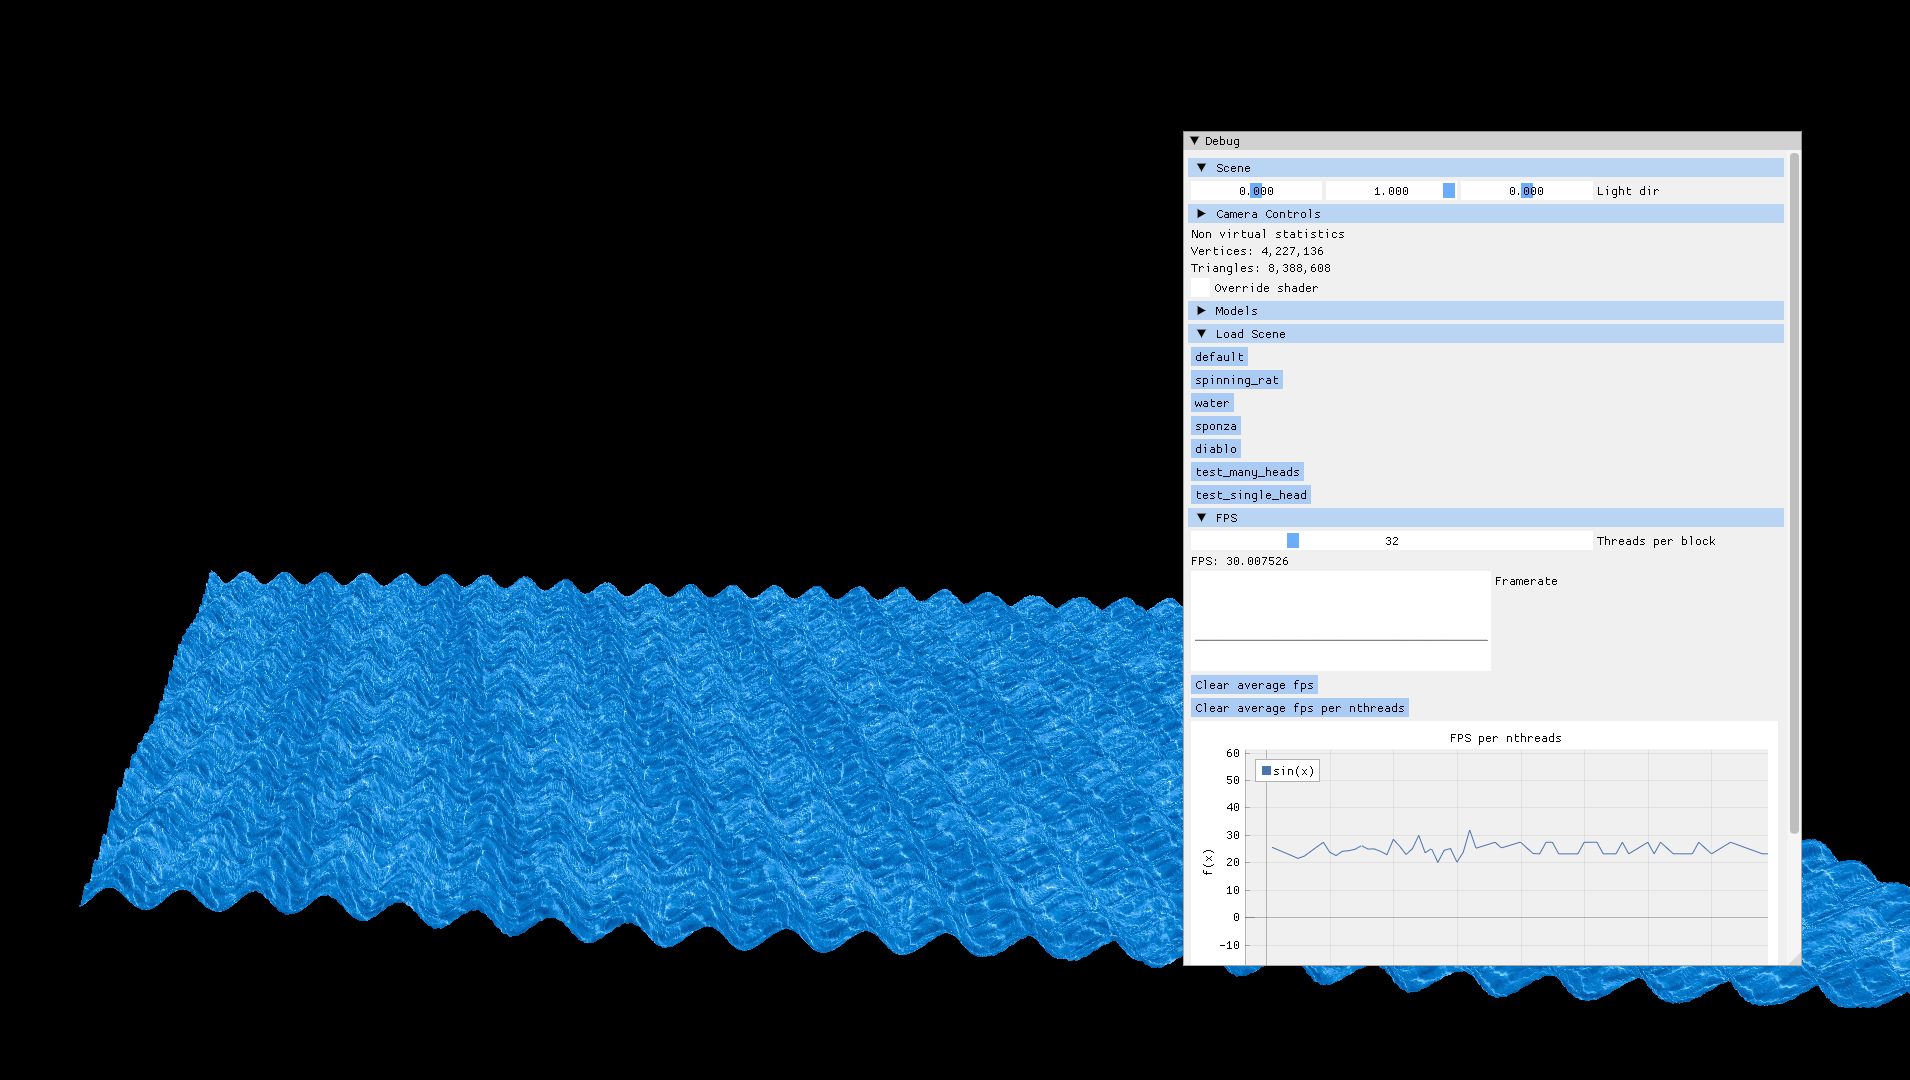
\includegraphics[scale=0.3]{img/interface.png}
	\end{center}
	\captionsetup{justification=centering}
	\caption{Идея работы алгоритма параллельной редукции}
	\label{img:program_interface_basic}
\end{figure}

Интерфейс состоит из секций:
\begin{itemize} 
	\item секция ''Scene''
		 \begin{itemize} 
			\item слайдер ''Light Dir'' -- контролирует направление источника освещения
			\item секция ''Camera Controls''
				\begin{itemize}
					\item слайдер ''Camera XY'' -- XY координаты камеры;
					\item слайдер ''Camera Z'' -- Z координаты камеры;
					\item слайдер ''Look dir yaw'' -- угол камеры по горизонтали;
					\item  слайдер ''Look dir pitch'' -- угол камеры по вертикали;
					\item слайдер ''FOV'' -- параметр поля зрения камеры
					\item слайдер ''zFar'' -- крайняя координата z пирамиды видимости для обрезки моделей;
				\end{itemize}
			\item заголовок ''Non virtual statistics'' -- статистика невиртуальных моделей - количество отрисовываемых граней и вершин;
			\item чекбокс ''Override Shader'' и выбор Shader - выбрать глобальный шейдер для использования всеми объектами сцены.
		 \end{itemize}
	\item секция ''Models'' -- содержит список объектов
		 \begin{itemize}
			\item слайдер ''Position'' -- позиция модели на сцене;
			\item выбор ''Shader'' -- шейдер, который использует модель;
		 \end{itemize}
	\item секция ''Load Scene'' -- содержит список предопределенных сцен для загрузки;
	\item секция ''FPS'' -- содержит информацию о производительности (кадрах в секунду)
		 \begin{itemize}
			\item слайдер ''Threads per Block'' -- слайдер с выбором кол-ва потоков, которые будут использовать Cuda kernel;
			\item график ''FPS'' -- отображает кол-во кадров в секунду;
			\item кнопки ''Clean X'' -- очищают график ''FPS per nthreads'';
			\item график ''FPS per nthreads'' -- по оси X - кол-во кадров, по Y - кол-во фпс (среднее);
		 \end{itemize}
	\item секция ''Culling'' -- содержит настройки удаления полностью невидимых объектов (куллинга)
		 \begin{itemize}
			\item чекбокс ''Enable Culling'' -- включает удаление невидимых объектов;
			\item заголовок ''Called to draw models: n'' -- n - кол-во объектов поступивших на отрисовку;
			\item заголовок ''Drawn after culling: n'' -- n - кол-во отрисованных объектов;
			\item график ''Culling Percentage'' -- по оси X - время, по оси Y - процент отброшенных объектов;
		 \end{itemize}
	\item секция ''Virtual Geometry'' -- виртуальная геометрия
		 \begin{itemize}
			\item слайдер ''Threshold'' -- площадь грани в пикселах, после которого она будет дробиться на подграни;
		 \end{itemize}
\end{itemize}

\section{Результаты работы программного обеспечения}

На рисунке \ref{img:t1} приведен результат отрисовки модели головы.

\begin{figure}[H]
	\begin{center}
		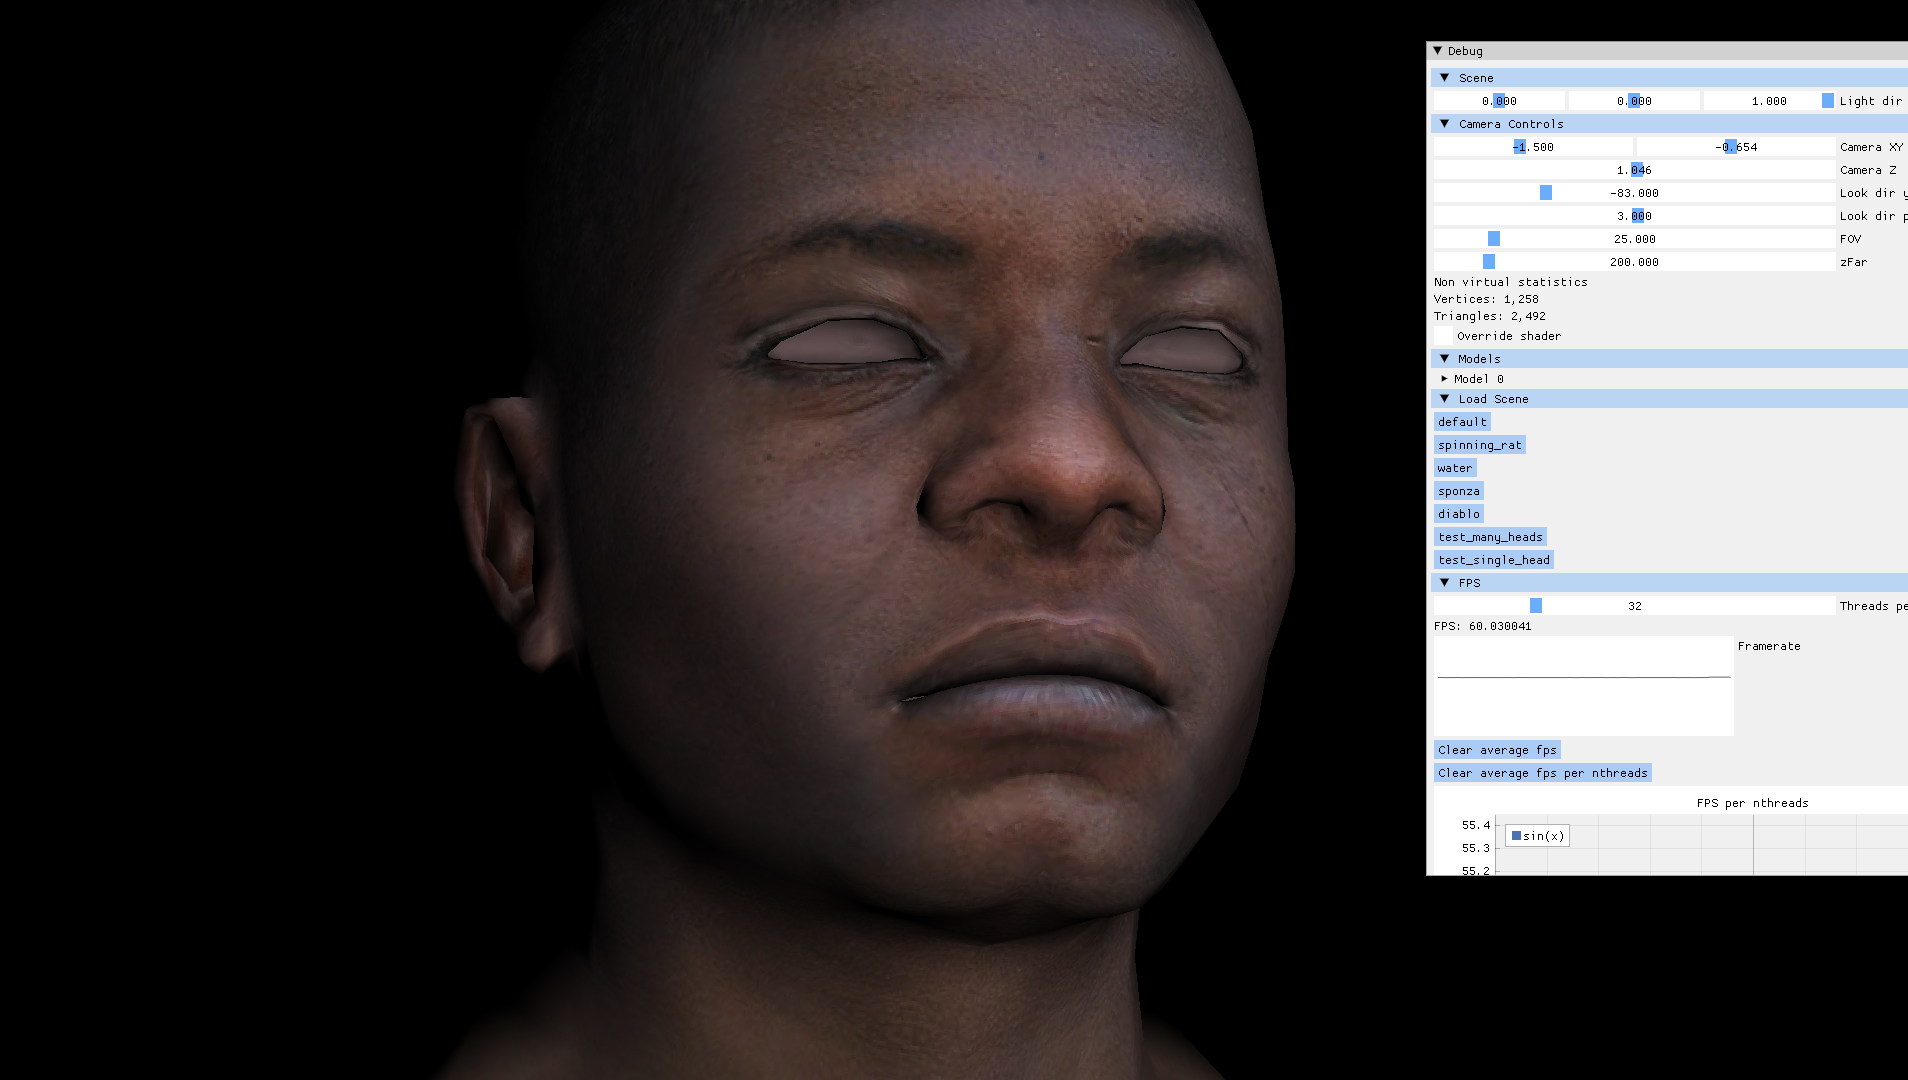
\includegraphics[scale=0.3]{img/i1.png}
	\end{center}
	\captionsetup{justification=centering}
	\caption{Модель головы}
	\label{img:t1}
\end{figure}

На рисунке показана тта же голова, вблизи. Видна проблема разных площадей граней, видимые артефакты на шее.
Это связано с тем, что их площадь слишком большая, и алгоритм растеризации попросту останавливается, не дорисовывая эти грани.
Количество кадров в секунду (FPS) равно 30.

На рисунке \ref{img:vgeom_model_bad} представлен вид геометрии объекта. Видны треугольники больших площадей, с теми же артефактами.

На рисунке \ref{img:vgeom_model_good} включена виртуальная геометрия. Число треугольников увеличилось, артефакты  пропали.

Рисунок \ref{img:vgeom_model_good_original_shader} показывает ту же модель, при ее обычном шейдере, без артефактов, с обновленной виртуальной геометрией.
При этом количество кадров возрастает до 60. Можно менять положение камеры и при этом наблюдать изменение виртуальной геометрии в реальном времени. 

\begin{figure}[H]
	\begin{center}
		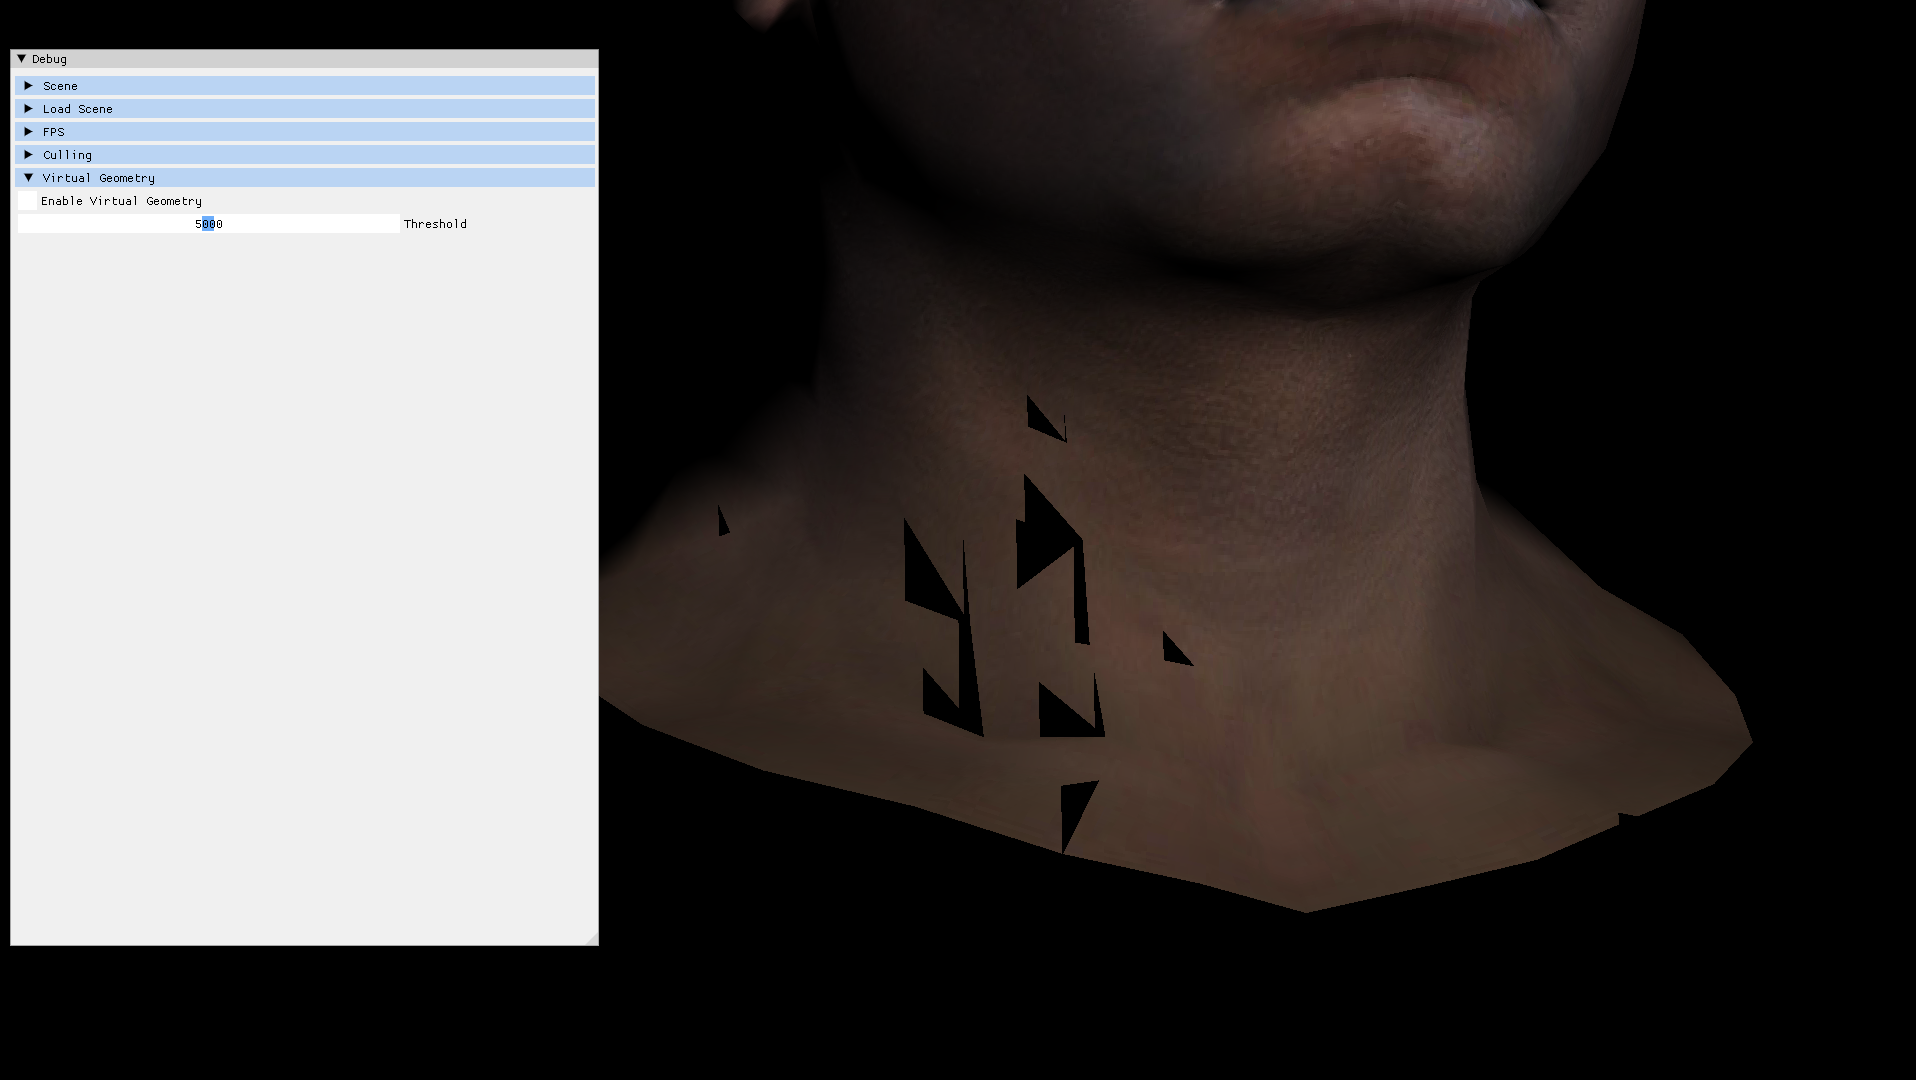
\includegraphics[scale=0.3]{img/i5.png}
	\end{center}
	\captionsetup{justification=centering}
	\caption{Модель головы вблизи, видны артефакты из-за разности площадей грани} 
	\label{img:vgeom_original_model_bad}
\end{figure}

\begin{figure}[H]
	\begin{center}
		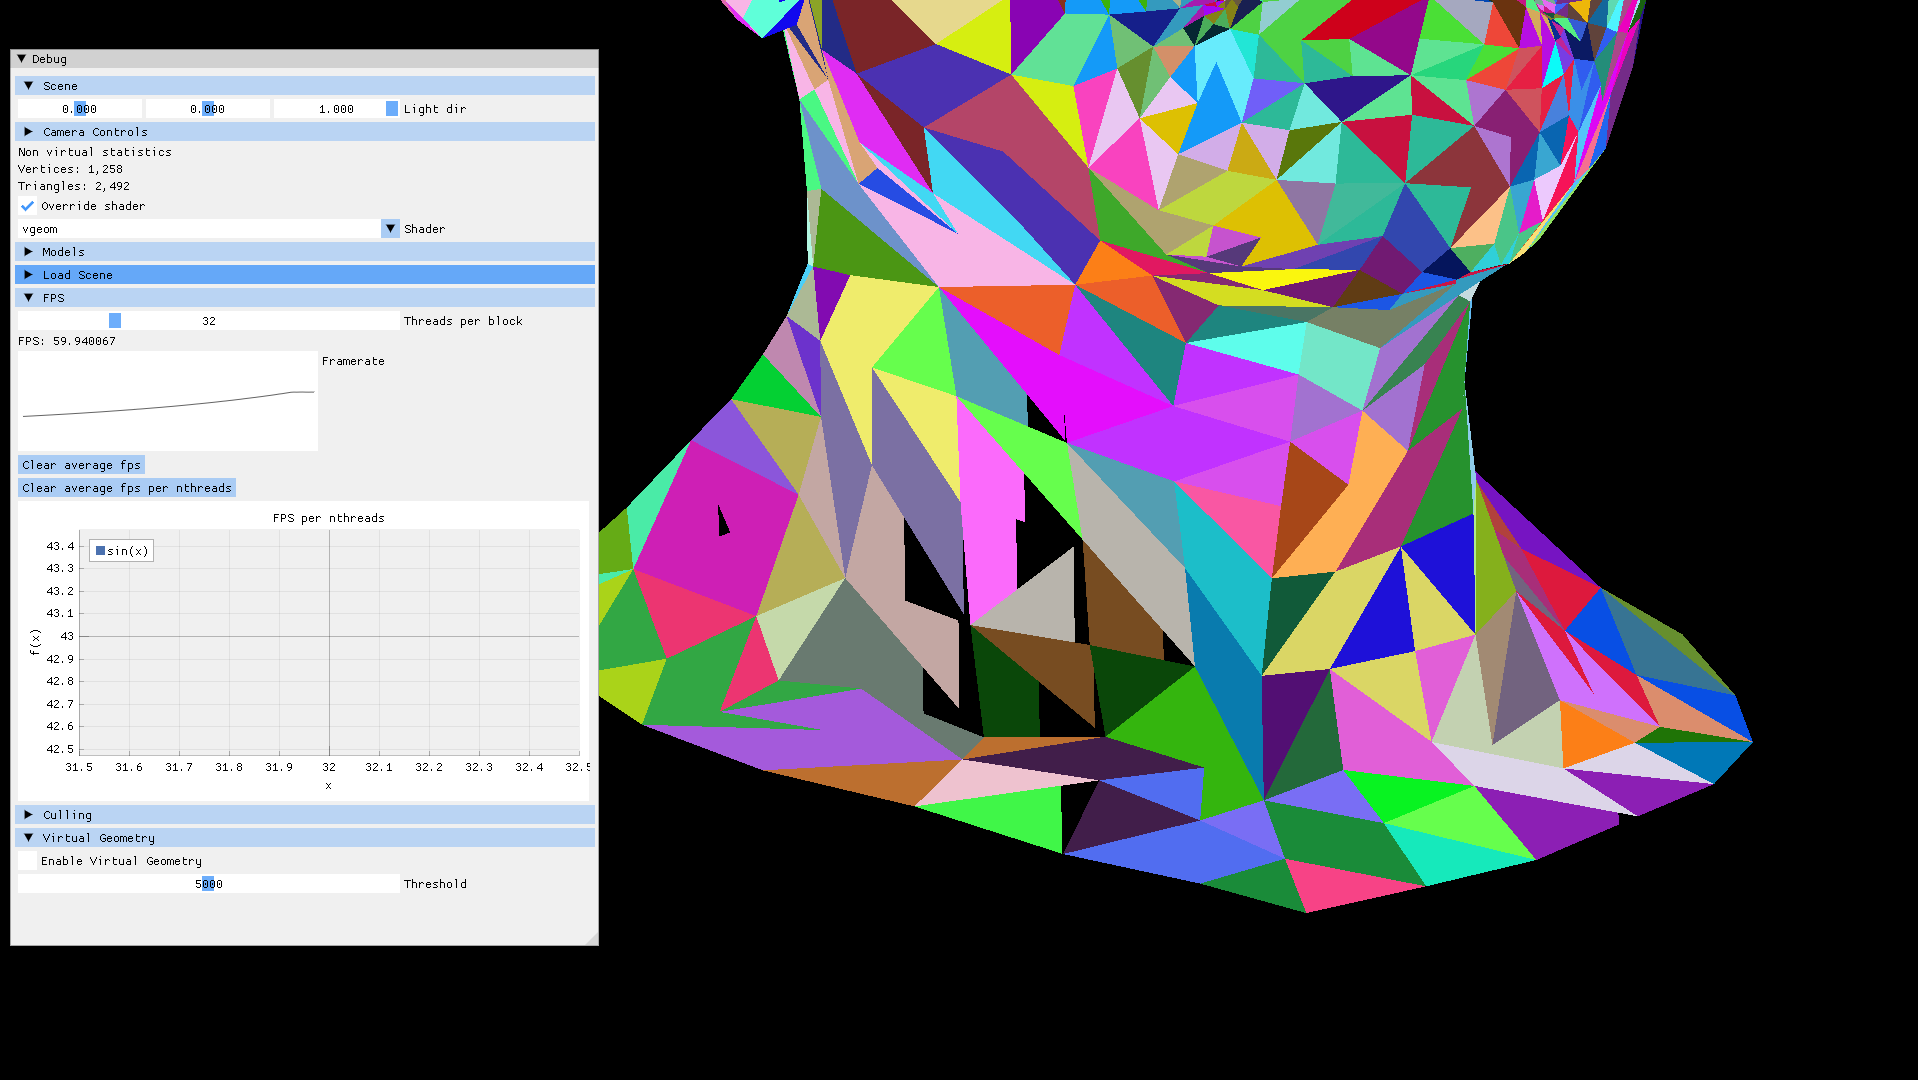
\includegraphics[scale=0.3]{img/vgeom_view_bad.png}
	\end{center}
	\captionsetup{justification=centering}
	\caption{Модель головы вблизи, геометрический шейдер, видны артефакты из-за разности площадей грани} 
	\label{img:vgeom_model_bad}
\end{figure}

\begin{figure}[H]
	\begin{center}
		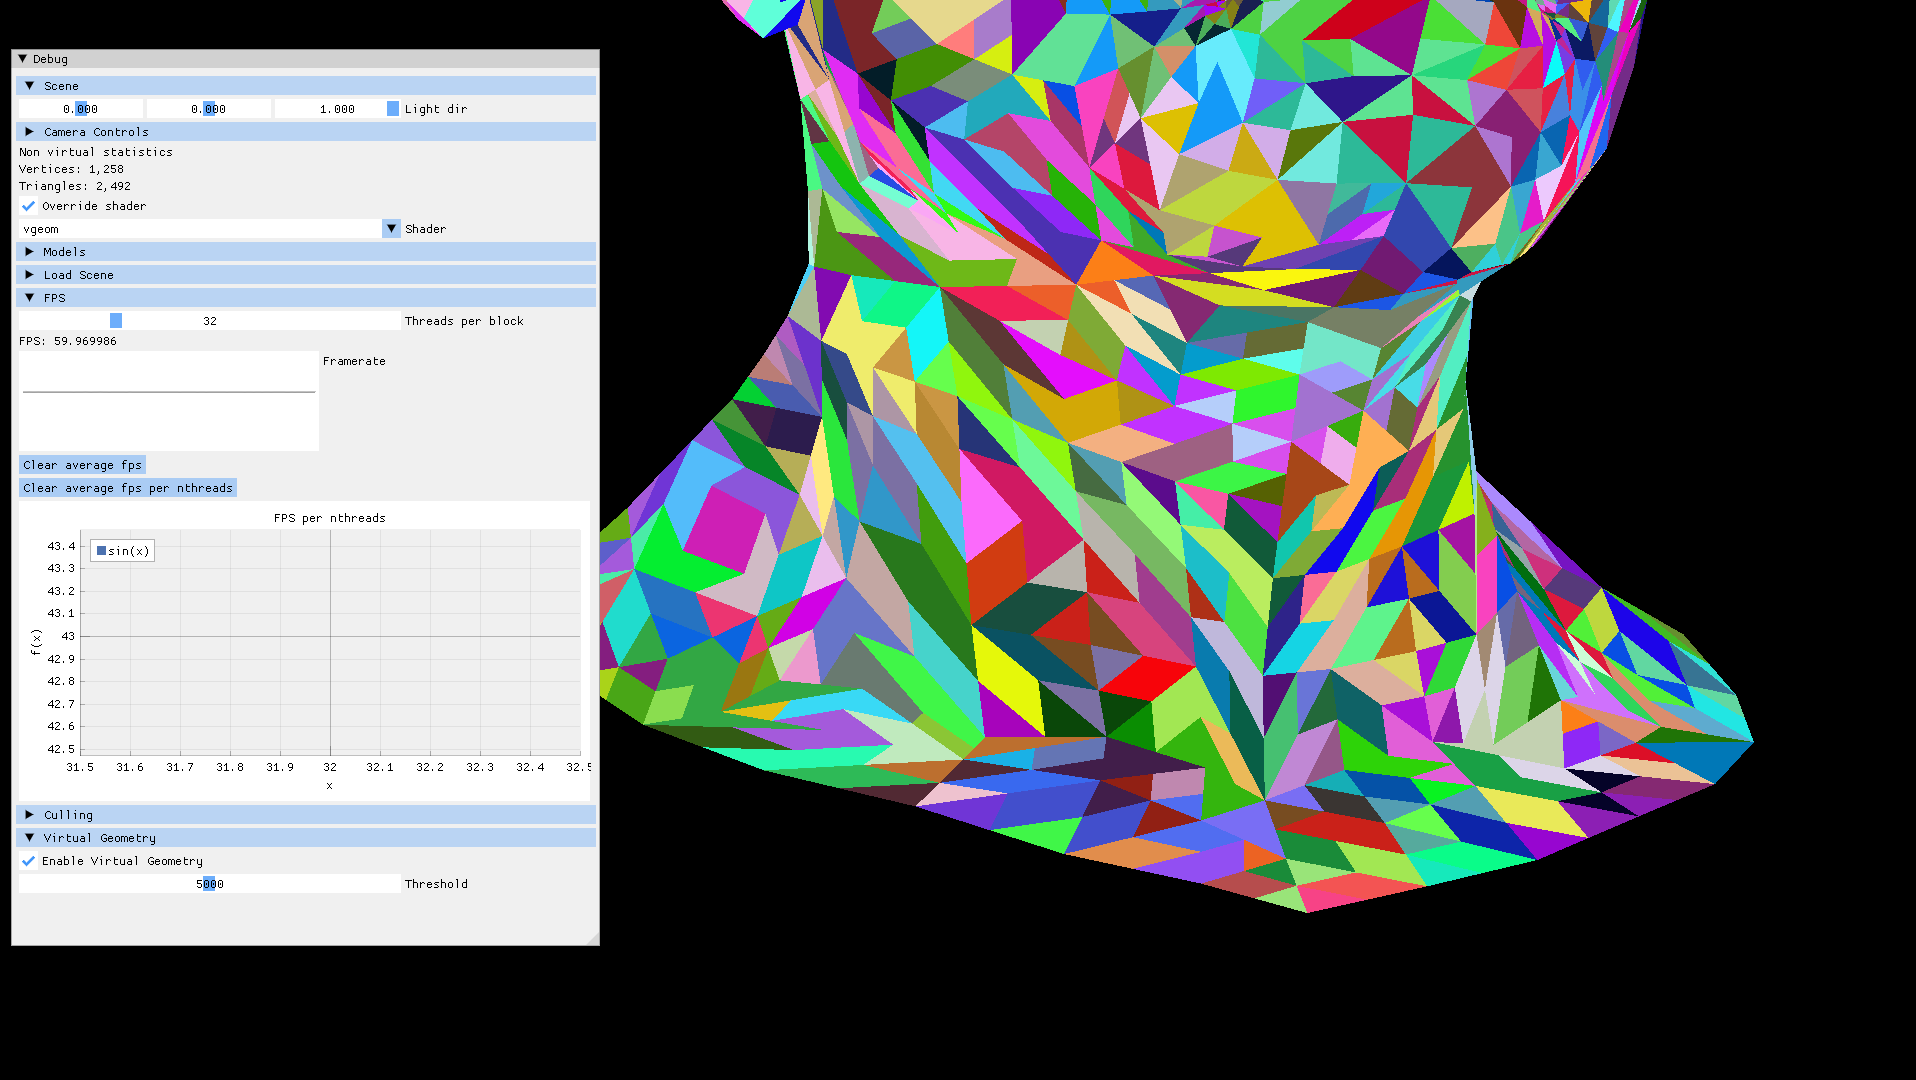
\includegraphics[scale=0.3]{img/vgeom_view_good.png}
	\end{center}
	\captionsetup{justification=centering}
	\caption{Модель головы вблизи, геометрический шейдер, при виртуальной геометрии число треугольников увеличилось, а артефакты пропали. } 
	\label{img:vgeom_model_good}
\end{figure}

\begin{figure}[H]
	\begin{center}
		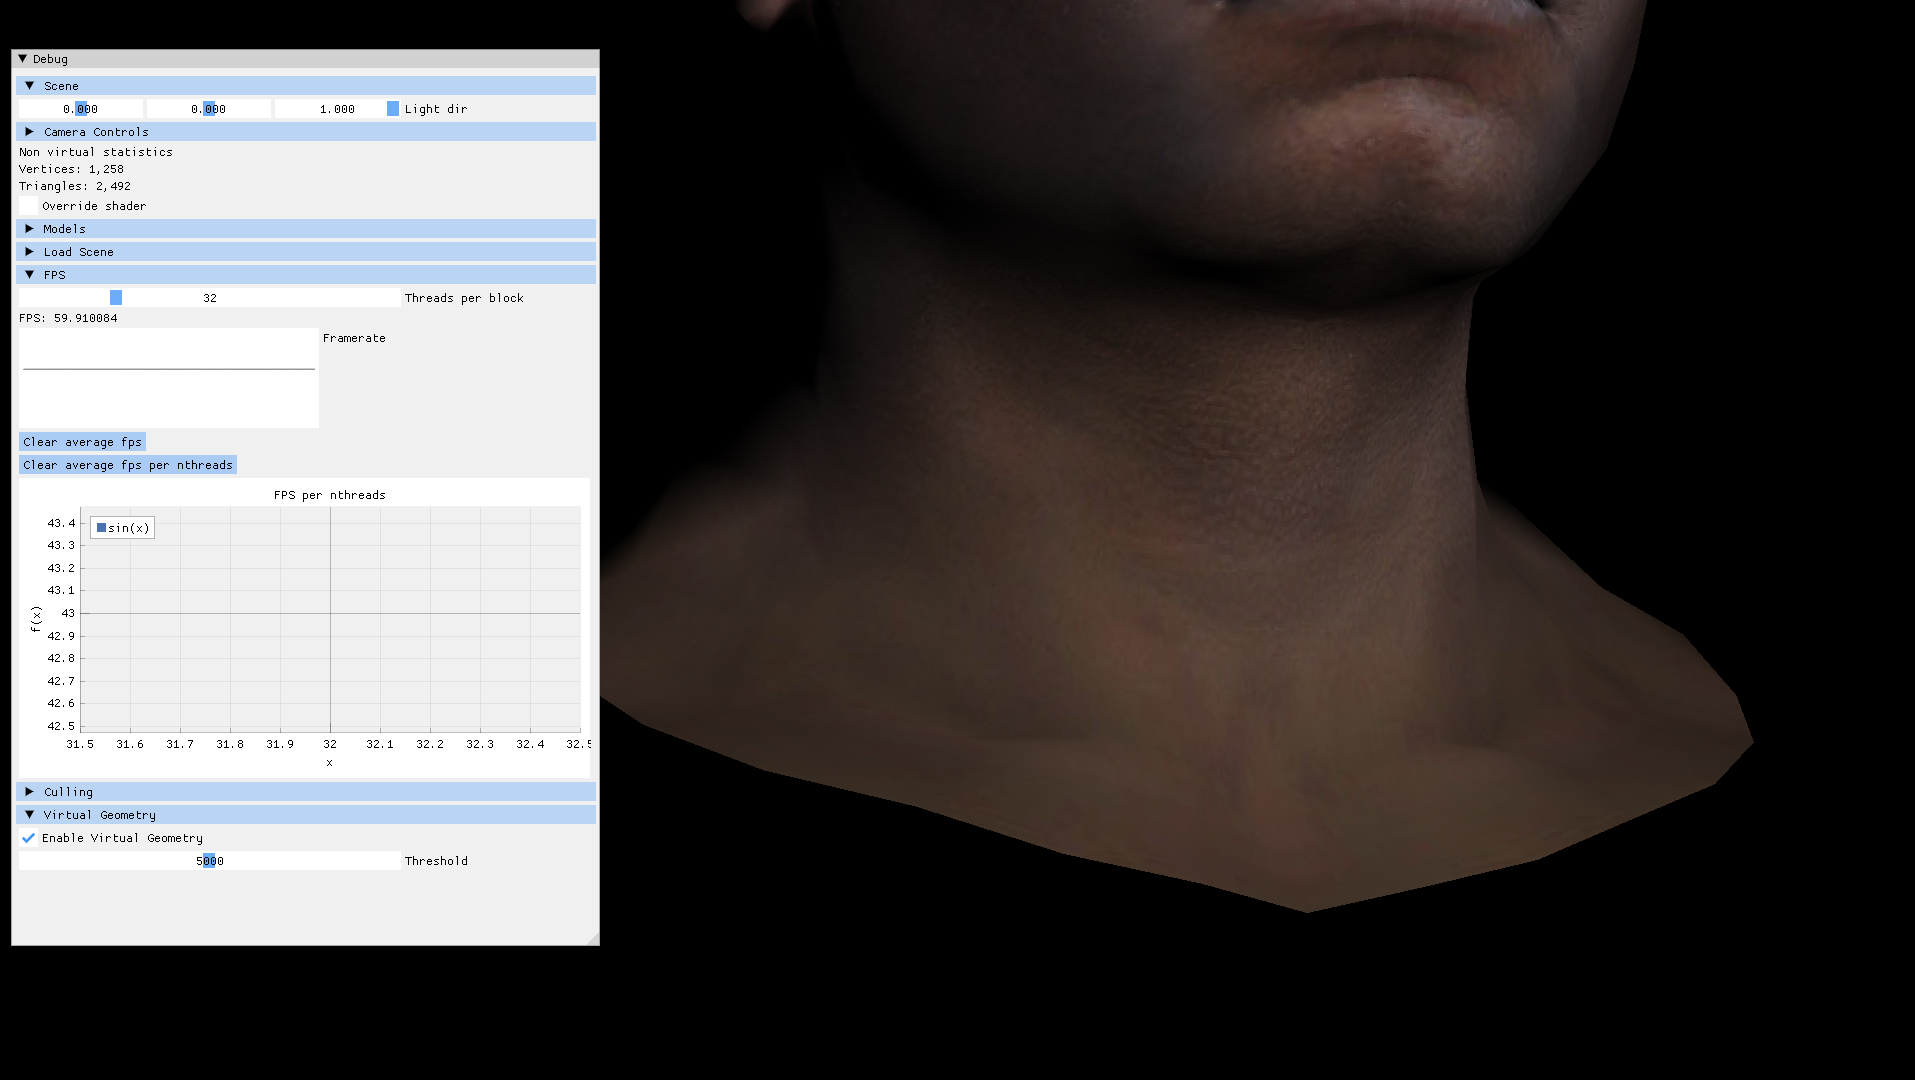
\includegraphics[scale=0.3]{img/vgeom_original_model.png}
	\end{center}
	\captionsetup{justification=centering}
	\caption{Модель головы вблизи, при виртуальной геометрии, артефакты пропали а FPS возрос. } 
	\label{img:vgeom_model_good_original_shader}
\end{figure}

\begin{figure}[H]
	\begin{center}
		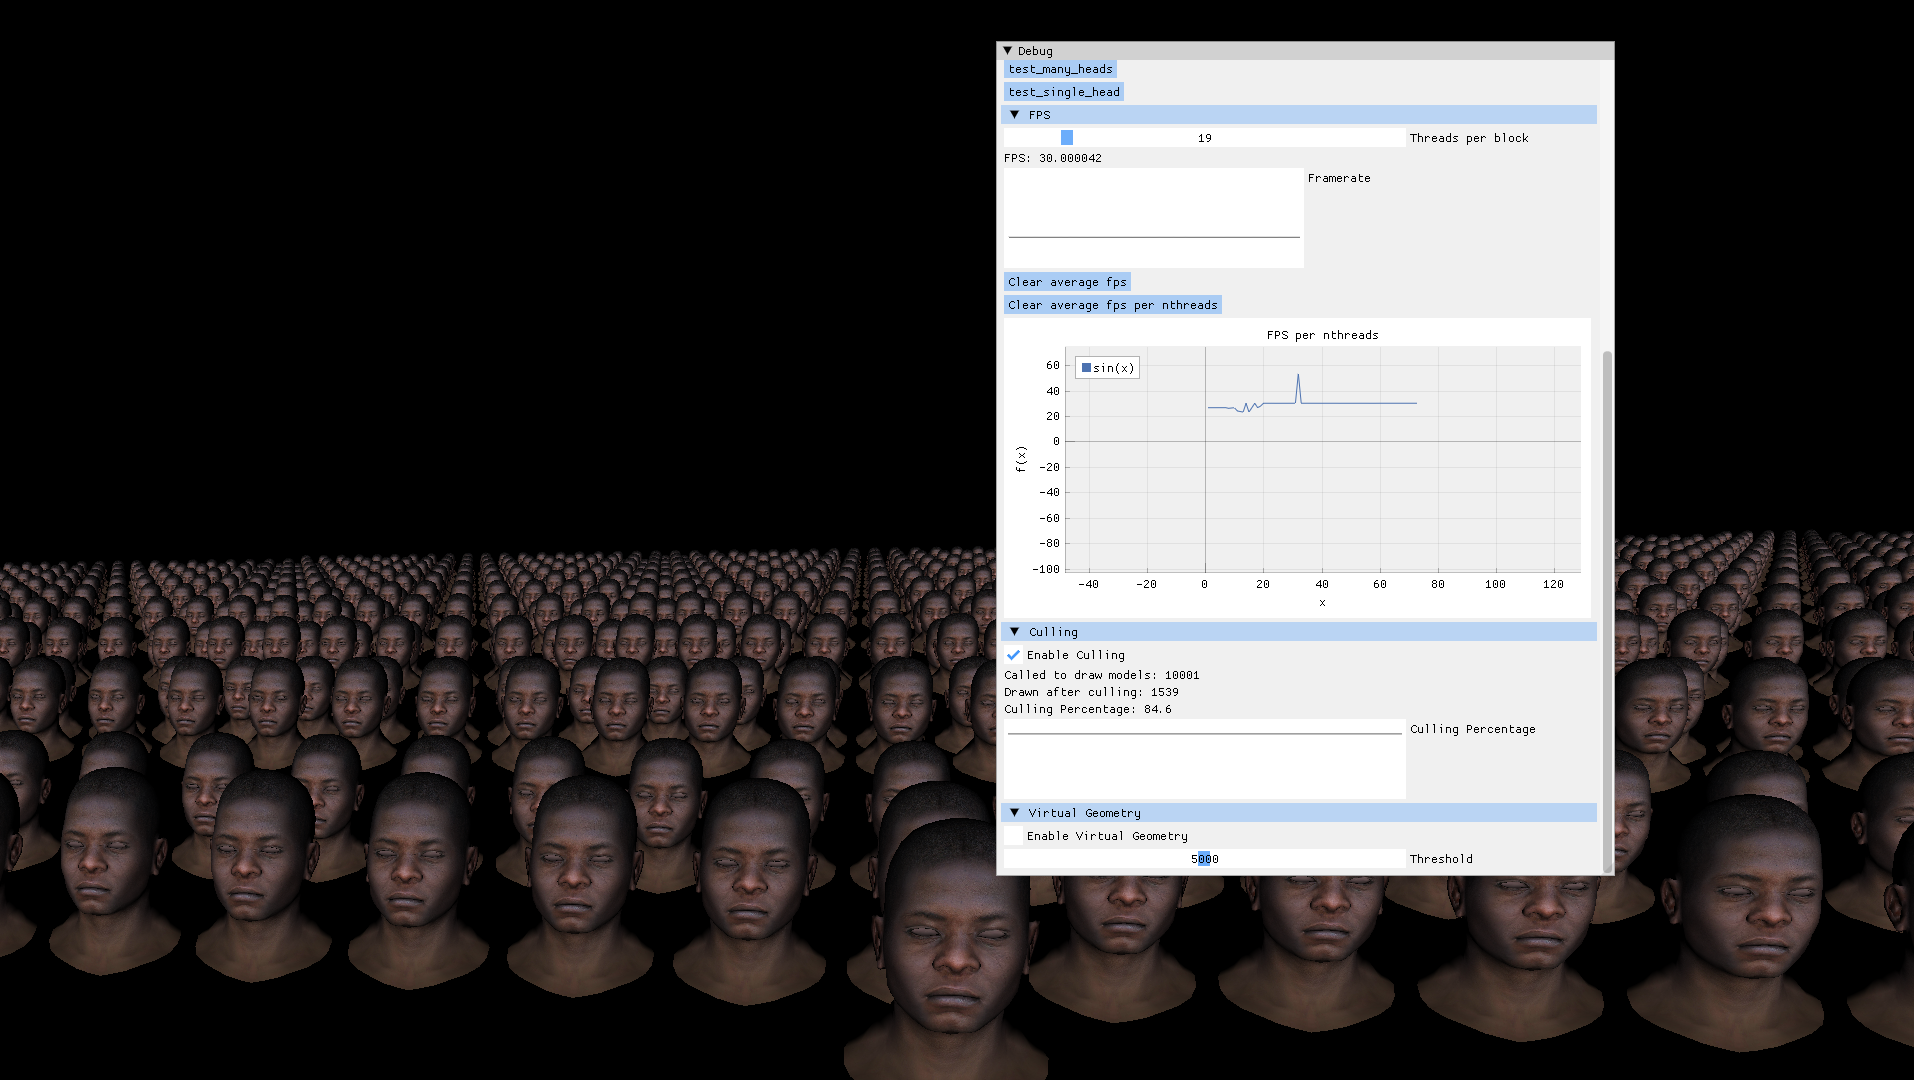
\includegraphics[scale=0.30]{img/i2.png}
	\end{center}
	\captionsetup{justification=centering}
	\caption{Отрисовка 10.000 объектов (30 FPS при Culling, 20 без)}
	\label{img:10k_negroes}
\end{figure}

\begin{figure}[H]
	\begin{center}
		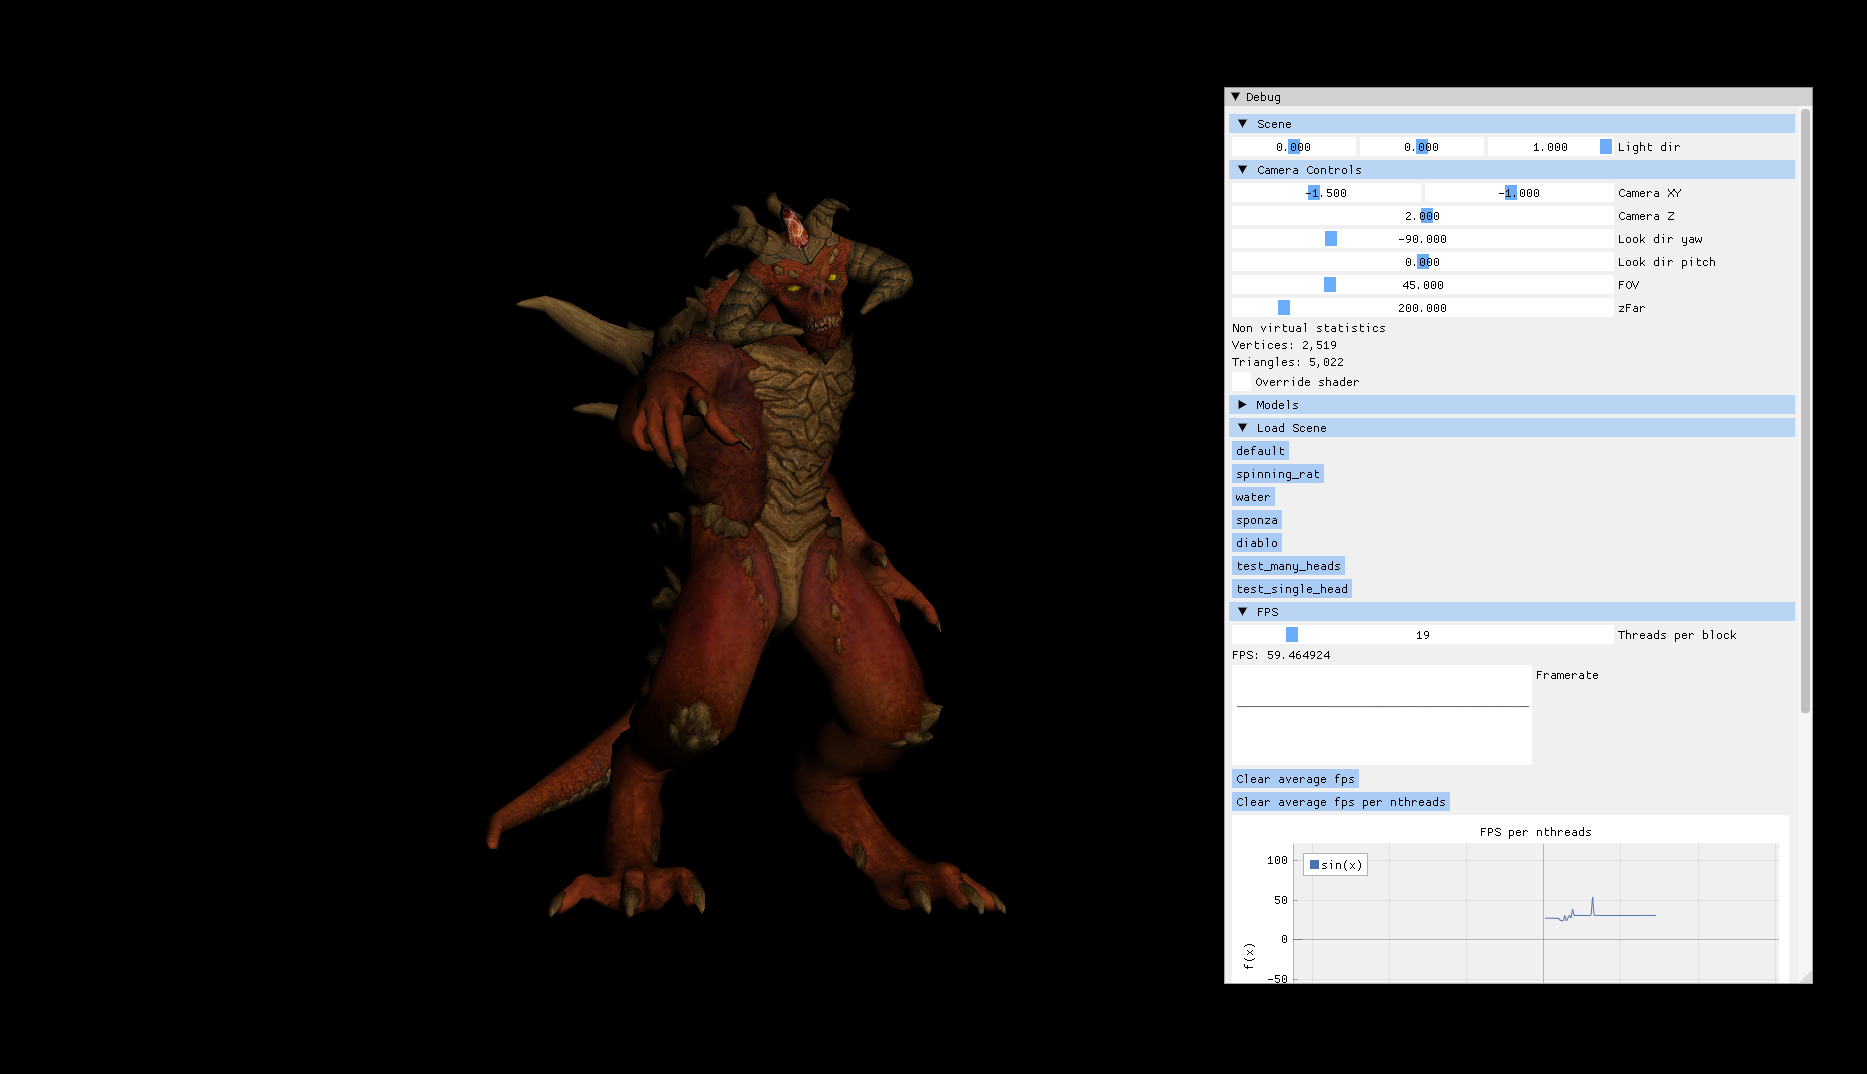
\includegraphics[scale=0.30]{img/i4.png}
	\end{center}
	\captionsetup{justification=centering}
	\caption{Модель персонажа Diablo}
	\label{img:diablo}
\end{figure}

\begin{figure}[H]
	\begin{center}
		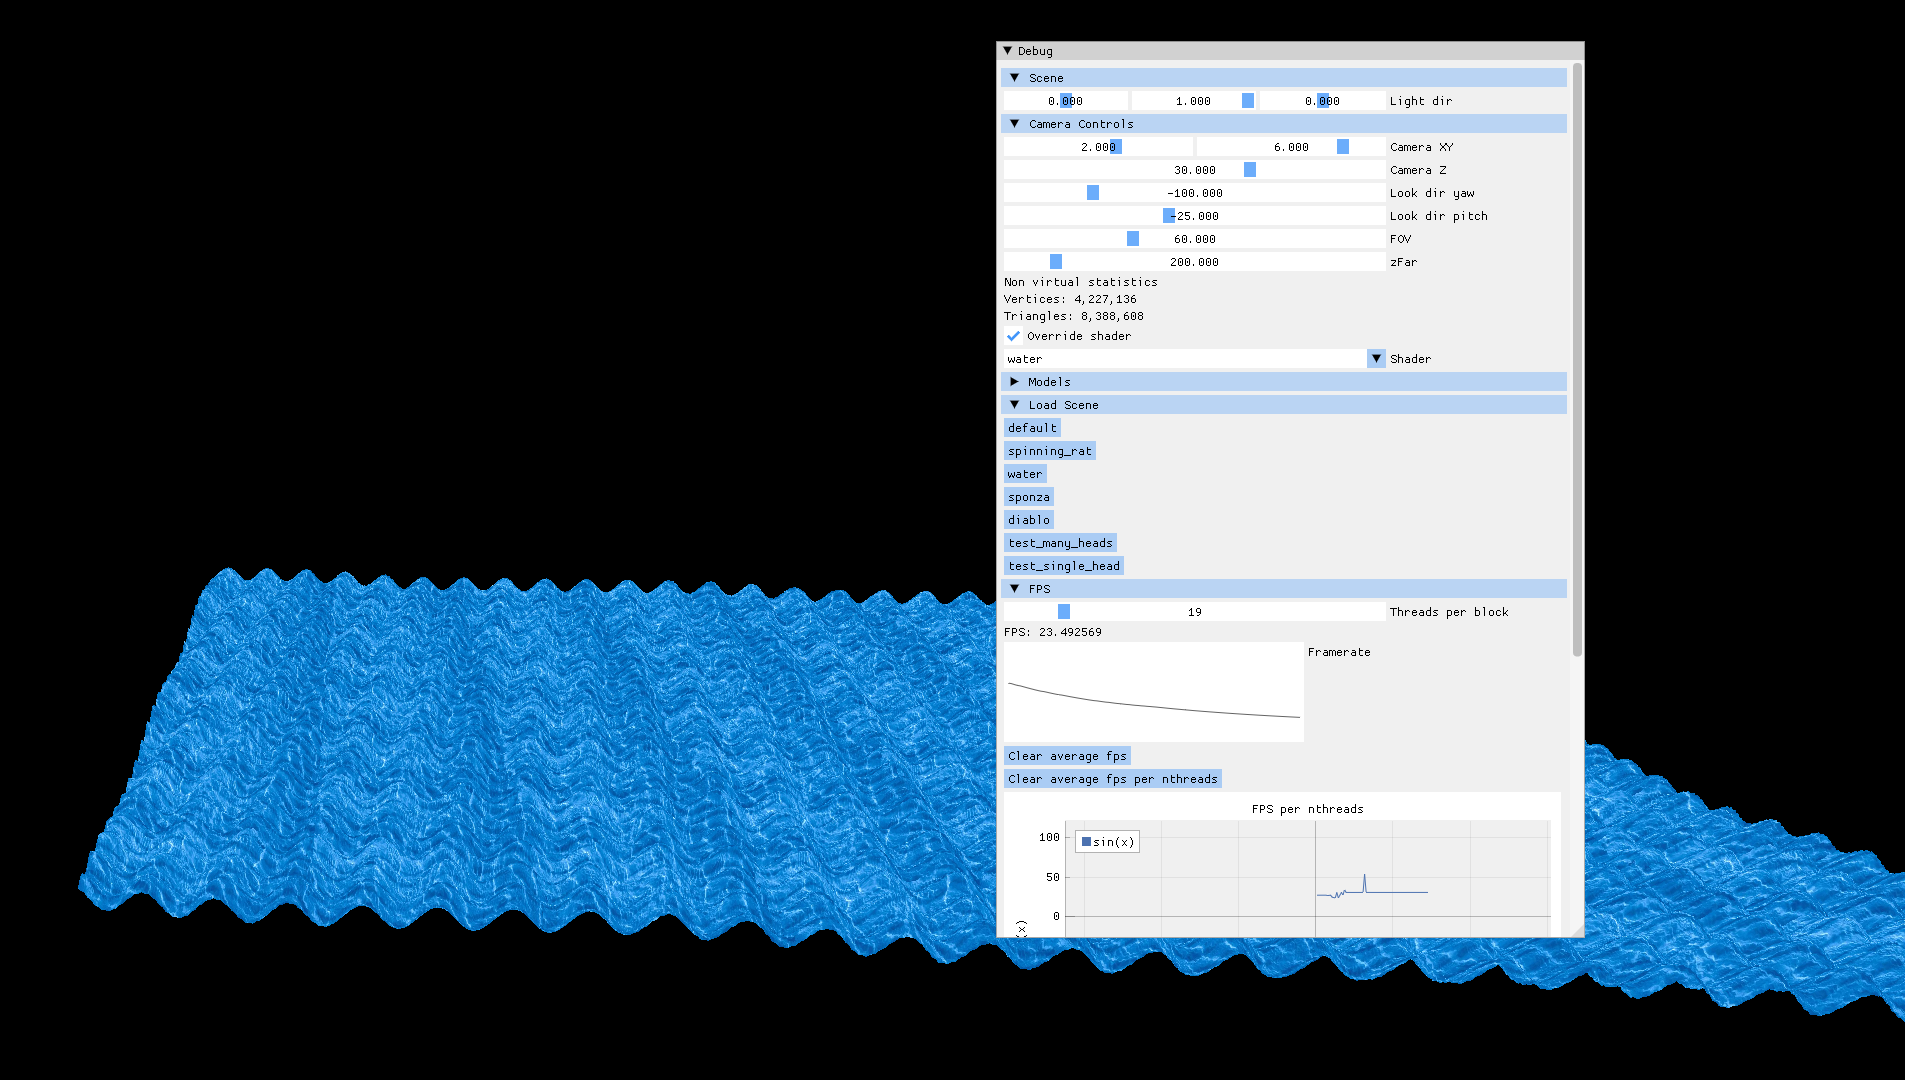
\includegraphics[scale=0.30]{img/i3.png}
	\end{center}
	\captionsetup{justification=centering}
	\caption{Вершинный шейдер воды}
	\label{img:water}
\end{figure}

Рисунок \ref{img:water} показывает работу вершинного шейдера воды.

\section*{Вывод}
В этом разделе был выбран язык программирования и среда разработки, представлен код вызова отрисовки, подробно разобран интерфейс приложения и приведены результаты работы программы.